\documentclass[tikz,border=8pt]{standalone}
\usepackage{amsmath}
\usetikzlibrary{arrows.meta,positioning,shapes.geometric}
\begin{document}
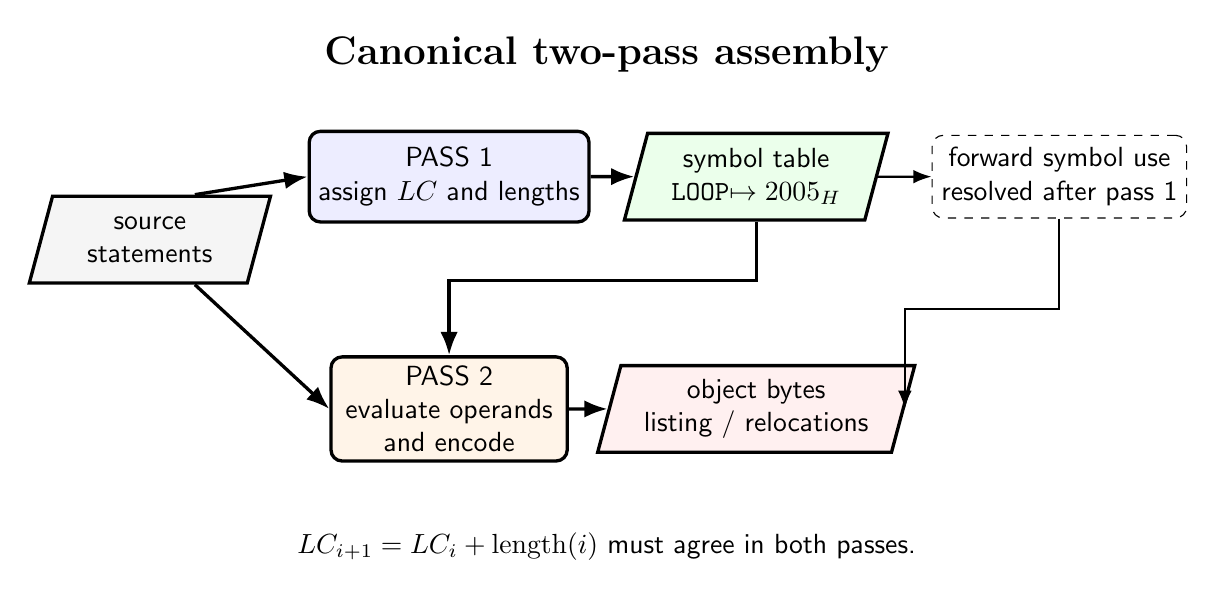
\begin{tikzpicture}[font=\sffamily,>=Latex,
 box/.style={draw,very thick,rounded corners,minimum width=3.0cm,minimum height=1.15cm,align=center},
 data/.style={draw,very thick,trapezium,trapezium left angle=75,trapezium right angle=105,minimum width=2.8cm,minimum height=1.1cm,align=center}]
\node[font=\Large\bfseries] at (7.25,6.55) {Canonical two-pass assembly};
\node[data,fill=gray!8] (src) at (1.45,4.2) {source\\statements};
\node[box,fill=blue!7] (p1) at (5.25,5.0) {PASS 1\\assign $LC$ and lengths};
\node[data,fill=green!8] (sym) at (9.15,5.0) {symbol table\\\texttt{LOOP}$\mapsto2005_H$};
\node[box,fill=orange!9] (p2) at (5.25,2.05) {PASS 2\\evaluate operands\\and encode};
\node[data,fill=red!6] (out) at (9.15,2.05) {object bytes\\listing / relocations};
\draw[very thick,->] (src.north east)--(p1.west);
\draw[very thick,->] (p1)--(sym);
\draw[very thick,->] (src.south east)--(p2.west);
\draw[very thick,->] (sym.south)--++(0,-.75)-|(p2.north);
\draw[very thick,->] (p2)--(out);
\node[draw,dashed,rounded corners,align=center,minimum width=2.8cm,minimum height=1.05cm] (fwd) at (13.0,5.0) {forward symbol use\\resolved after pass 1};
\draw[thick,->] (sym)--(fwd);
\draw[thick,->] (fwd.south)--++(0,-1.15)-|(out.east);
\node at (7.25,.3) {$LC_{i+1}=LC_i+\operatorname{length}(i)$ must agree in both passes.};
\end{tikzpicture}
\end{document}
